\documentclass[12pt,a4paper,twoside]{article}
\usepackage{polski}
\usepackage[utf8]{inputenc}
\usepackage[left=3.5cm,right=2.5cm,top=2.5cm,bottom=2.5cm]{geometry}
\usepackage{graphicx}
\usepackage{lipsum}
\usepackage{setspace}
\usepackage{xcolor}
\spacing{1.5}
\setlength{\parindent}{1.25cm}
%% ########################################################
\begin{document}
\thispagestyle{empty}
\begin{center}

\includegraphics[width=\textwidth]{img/logo_AGH.jpg}\\
{\bf{\sf WYDZIAŁ GEOLOGII, GEOFIZYKI I OCHRONY ŚRODOWISKA}}\\[5mm]
%% ======================================================
{\bf{\sf{KATEDRA GEOINFORMATYKI I INFORMATYKI STOSOWANEJ}}}\\[14mm]

{\sf{\huge Projekt dyplomowy}}\\[12mm] 
%% ======================================================
{\sf{\Large Aplikacja do zarządzania zbiorami danych\\[2mm] 
Dataset management application}}\\[40mm]
\end{center}
{\sf\begin{tabular}{ll}
	Autor: & Monika Hertel\\
	Kierunek studiów: & Inżynieria i Analiza Danych\\
	Opiekun pracy: & dr Paweł Oleksik\\
\end{tabular}}\\[10mm]
\begin{center}
{\sf Kraków, 2024}
\end{center}
%% ########################################################
\newpage
\tableofcontents
\newpage
\section*{Wstęp}
\addcontentsline{toc}{section}{Wstęp}
Dane odgrywają niezwykle istotną rolę w funkcjonowaniu współczesnego społeczeństwa, będąc fundamentem dla wielu procesów i decyzji. Dzięki danym można analizować i rozumieć zmiany w otaczającym świecie, identyfikować wzorce i trendy oraz przewidywać przyszłe wydarzenia.\par
Przechowywanie danych jest niezbędne nie tylko ze względu na konieczność zachowania informacji historycznych, ale także po to, aby zapewnić dostępność potrzebnych informacji w odpowiednim czasie oraz miejscu. Organizacje różnego rodzaju gromadzą ogromne ilości informacji, które są kluczowe dla ich funkcjonowania i rozwoju. Systematyczne przechowywanie tych danych pozwala na śledzenie zmian w czasie, analizę trendów oraz identyfikację ważnych wzorców i relacji, co z kolei umożliwia podejmowanie trafniejszych decyzji biznesowych. Wykorzystując dane, można personalizować doświadczenia użytkowników, dostosowując produkty i usługi do ich potrzeb i preferencji.\par
W kontekście poniższej pracy, zbiór danych jest określany jako plik zawierający w sobie wszelkie informacje, tj. artykuły naukowe, dane tabelaryczne, grafiki czy notatki. Każdy z tych przykładów przechowuje wiedzę możliwą do interpretacji przez człowieka. Do przeprowadzenia analizy danych, często potrzebna jest znajomość teorii kryjącej się za wartościami w zestawie.\par
Zapewnienie bezpieczeństwa i poufności gromadzonych informacji jest również ważnym aspektem przechowywania danych. W obliczu coraz częstszych przypadków naruszeń danych i cyberataków, odpowiednie zabezpieczenie przechowywanych danych staje się priorytetem. Dlatego też organizacje, ale także osoby prywatne muszą inwestować w zaawansowane systemy ochrony danych i stosować odpowiednie procedury zarządzania dostępem do informacji.\par
\subsection*{Cel i zakres projektu}
Projekt ma na celu przedstawienie możliwości systemu ułatwiającego użytkownikowi proces zbierania i segregowania informacji. Poniższa praca skupi się na zaprezentowaniu konceptu aplikacji oraz szczegółowym opisie implementacji modułu obsługi artykułów.
\newpage
%% ########################################################
\section{Zagadnienia teoretyczne}
Zaprojektowany system ma uprościć proces gromadzenia informacji dla użytkownika prywatnego. Zgromadzone dane mogą być przechowywane w pliku w systemie plików lub przy użyciu takich narzędzi jak bazy danych. Rozważając rodzaj przechowywania danych należy również wziąć pod uwagę aspekt fizyczny. Rozróżnienie to jest opisane w rozdziale 1.1. Wraz z danymi będą przechowywanie metainformacje, opisujące te dane.  \par
Pozyskiwanie informacji z plików różni się zależnie od ich rodzaju. Aplikacja umożliwia przetworzenie plików tabelarycznych czy tekstowych, poprzez wykorzystanie ich zawartości. Szczególnym przypadkiem są pliki PDF, gdzie proces ekstrakcji zawartości jest utrudniony w związku z kodowaniem i formatem pliku, co zostanie omówione w dziale 1.2. \par
Analiza tekstu może być przeprowadzona pod kilkoma względami\par
Projekt aplikacji wykorzystuje architekture typu klient-serwer, jednakże dzięki wykorzystaniu pakietu \textit{Electron} języka Javascript, jest możliwe przekształcenie aplikacji webowej na natywną. Biblioteka Electron jest projektem umożliwiającym tworzenie aplikacji natywnych używając technologii web. Pełny opis tej biblioteki jest zawarty w podrozdziale 1.4. 
%% ########################################################
%% 
\subsection{Sposoby przechowywania informacji}
Istnieje wiele sposobów magazynowania danych. Wybór odpowiedniego sposobu zależy od indywidualnych potrzeb użytkownika oraz od ilości informacji. Na poziomie organizacji dzielą się one na serwery lokalne (\textit{ang. on-premises servers}) oraz przechowywanie w chmurze (\textit{ang. cloud storage}). Poniżej zostały opisane obie metody.\par
Pojęcie \textbf{serwerów on-premises} odnosi się do fizycznego sprzętu i infrastruktury, które znajdują się pod kontrolą organizacji lub osoby fizycznej. Podejście to obejmuje konfigurowanie i utrzymywanie serwerów na miejscu w celu przechowywania danych i zarządzania nimi, bez angażowania usługodawców zewnętrznych. Oto przegląd zalet i wad korzystania z serwerów lokalnych do przechowywania danych:
\begin{itemize}
	\item zalety:
		\begin{enumerate}
			\item Bezpośrednia kontrola - Organizacje mają pełną kontrolę nad swoim sprzętem i oprogramowaniem, co pozwala na większą elastyczność zarządzania w celu spełnienia określonych potrzeb biznesowych i wymogów bezpieczeństwa.
			\item Bezpieczeństwo - Serwery lokalne zapewniają  wyższy poziom bezpieczeństwa i prywatności danych, ponieważ mogą one wdrażać własne środki bezpieczeństwa i protokoły dostosowane do ich konkretnych potrzeb. Może to obejmować fizyczne środki bezpieczeństwa, takie jak ograniczony dostęp do serwerowni i budynków.
			\item Zgodność z wymaganiami - W przypadku branż o surowych wymogach regulacyjnych, takich jak opieka zdrowotna lub finanse, serwery lokalne oferują lepszą kontrolę zgodności z nimi. Właściciele mogą zapewnić, że praktyki przetwarzania danych są zgodne z odpowiednimi regulacjami i przepisami.
			\item Personalizacja - Oferują one elastyczność w zakresie dostosowywania konfiguracji sprzętowych lub konfiguracji sieci w celu optymalizacji wydajności i spełnienia określonych wymagań dotyczących obciążenia.\\
		\end{enumerate}
	\item wady:
		\begin{enumerate}
			\item Koszty początkowe oraz utrzymania - Konfiguracja serwerów lokalnych wymaga znacznych inwestycji w sprzęt, licencje, konfigurację sieciowy i strukturalną. Może to obejmować koszty związane z zakupem serwerów, macierzy dyskowych, przełączników sieciowych czy systemów chłodzenia. Wymusza to również odpowiedzialność za bieżącą konserwację, zarządzanie oprogramowaniem serwerowym, co może wymagać dedykowanego personelu i zasobów IT. Obejmuje to zadania takie jak naprawy sprzętu fizycznego lub aktualizacje oprogramowania.
			\item Ograniczenia skalowalności - Należy zakupić dodatkowy sprzęt i rozszerzyć infrastrukturę, aby sprostać rosnącym potrzebom w zakresie przechowywania i przetwarzania danych. 
			\item Ograniczona redundancja geograficzna - serwery mogą nie mieć redundancji geograficznej, co oznacza, że dane są przechowywane w jednej lokalizacji i są podatne na zagrożenia, takie jak klęski żywiołowe, pożary lub inne nieprzewidziane zdarzenia, które mogą spowodować utratę danych.
		\end{enumerate}
\end{itemize}\par
Usługi \textbf{przechowywania w chmurze}, takie jak Amazon Web Services (AWS), zapewniają możliwość przechowywania danych i zarządzania nimi w zdalnych centrach danych utrzymywanych przez zewnętrznych dostawców usług. Poniżej przedstawiono przegląd wad i zalet korzystania z usług przechowywania danych w chmurze:
\begin{itemize}
	\item zalety:
		\begin{enumerate}
			\item Skalowalność: Usługi przechowywania danych w chmurze oferują praktycznie nieograniczoną skalowalność, umożliwiając organizacjom łatwe zwiększanie lub zmniejszanie pojemności pamięci masowej w zależności od zapotrzebowania. Ta elastyczność umożliwia firmom szybkie dostosowanie się do zmieniających się wymagań dotyczących pamięci masowej bez konieczności inwestowania z góry w sprzęt.
			\item Opłacalność: Pamięć w chmurze w większości przypadków działa w modelu cenowym pay-as-you-go, w którym organizacje płacą tylko za przestrzeń dyskową i zasoby, które wykorzystują. Może to prowadzić do oszczędności kosztów w porównaniu z tradycyjnymi lokalnymi rozwiązaniami.
			\item Dostępność: Zapewniają wszechobecny dostęp do danych z dowolnego miejsca z połączeniem internetowym. Umożliwia to zdalny dostęp, współpracę i udostępnianie danych między rozproszonymi zespołami, poprawiając produktywność oraz rozszerzając działalność firmy globalnie.
			\item Wysoka dostępność i niezawodność: Usługi przechowywania danych w chmurze zazwyczaj oferują wbudowane funkcje redundancji i wysokiej dostępności, zapewniając replikację danych w wielu centrach danych i ochronę przed awariami sprzętu lub innymi zakłóceniami. Skutkuje to zwiększoną niezawodnością danych i minimalnymi przestojami.
			\item Bezpieczeństwo: Wiodący dostawcy rozwiązań chmurowych wdrażają solidne środki bezpieczeństwa w celu ochrony danych, w tym szyfrowanie, kontrolę dostępu i certyfikaty zgodności.
		\end{enumerate}
	\item wady:
		\begin{enumerate}
			\item Zależność: Zależność od dostawcy usług w zakresie dostępności, bezpieczeństwa i wydajności danych. Wszelkie zakłócenia lub przerwy w świadczeniu usług po stronie dostawcy mogą mieć wpływ na dostęp do danych i operacje biznesowe.
			\item Zarządzanie danymi i zgodność z przepisami: Organizacje muszą upewnić się, że dane przechowywane w chmurze są zgodne z odpowiednimi przepisami i standardami.
			\item Koszty transferu danych: Podczas gdy przechowywanie danych w chmurze może być opłacalne, organizacje mogą ponieść dodatkowe koszty transferu danych, zwłaszcza w przypadku przenoszenia dużych ilości danych do i z chmury. Koszty mogą znacznie wzrosnąć w przypadku obciążeń wymagających dużej przepustowości.
			\item Problemy ze zmianą miejsca przechowywania: Migracja danych między dostawcami usług w chmurze lub powrót do infrastruktury lokalnej mogą być złożone i kosztowne. Organizacje ryzykują uzależnienie od dostawcy, gdy mocno inwestują w ekosystem określonego dystrybutora rozwiązań, co w dłuższej perspektywie ogranicza ich elastyczność.
			\item Obawy dotyczące bezpieczeństwa danych i prywatności: Pomimo solidnych środków bezpieczeństwa wdrożonych przez dostawców usług w chmurze, organizacje mogą nadal mieć obawy dotyczące bezpieczeństwa i prywatności swoich danych przechowywanych w chmurze.
		\end{enumerate}
\end{itemize}\par
Wybór miejsca przechowywania danych zależy od takich czynników, jak wymagania bezpieczeństwa, potrzeby skalowalności czy ograniczenia budżetowe. Często korzystne dla organizacji jest przyjęcie podejścia hybrydowego lub wielochmurowego, wykorzystującego mocne strony różnych opcji przechowywania danych. Umożliwia to zaspokojenie różnorodnych potrzeb biznesowych przy jednoczesnym złagodzeniu wpływu niedoskonałości różnych rozwiązań.
%% ########################################################
\subsection{Ekstrakcja tekstu plików PDF}
Pliki PDF są powszechnie przyjętym standardem przechowywania informacji. Format PDF jest oparty o strukturę binarnego formatu plików, zoptymalizowanego pod kątem wysokiej wydajności odczytu wizualnego. Zawierają w sobie informacje o strukturze dokumentu, takie jak zawartość tekstowa, grafiki czy użyta czcionka. Są one zoptymalizowane pod drukowanie. Niezaszyfrowane PDF mogą być w całości reprezentowane z użyciem wartości bitowych, odpowiadających części zbioru znaków zdefiniowanego w \textit{ANSI X3.4-1986}, symbole kontrolne oraz puste znaki. Wizualnie jednak nie są one ograniczone do zbioru znaków ASCII \cite{ISO32000}.\par
Format PDF separuje informacje dotyczące samego znaku a jego wizualną reprezentacją. Jest to rozróżnienie na znak pisarski i glif, gdzie grafem jest jednostką tekstu a glif, jednostką graficzną. Glif informuje o położeniu znaków na stronie dokumentu, jego czcionce i innych elementach wyglądu. \par
Otrzymanie zawartości pliku może być wykonane za pomocą wydobycia elementów PDF z strumienia pliku lub z użyciem analizy obrazów, na przykład technologi optycznego rozpoznawania znaków OCR (\textit{ang. Optical Character Recogintion}). 
Podstawowym zadaniem systemu OCR jest konwersja dokumentów w dane możliwe do edytowania czy wyszukiwania. Techniki oparte o analizę obrazów są bezpośrednio zależne od jakości wprowadzonego elementu. Idealną sytuacją dla wykożystania metod OCR jest kiedy posiadany plik zawiera w sobie jedynie tekst i jest obrazem binarnym \cite{mithe2013optical}. Dodatkowym atutem takich systemów jest możliwość wykrycia pisma i konwersja na tekst.\par
Ekstrahowanie danych z strumienia pliku, wiąże się z kilkoma problemami. Biorąc pod uwagę możliwość że plik pdf może posiadać różne kodowanie takie jak \textit{UTF-8}, \textit{ASCII} czy \textit{Unicode}, możemy doświadczyć utraty informacji spowodowanej schematem kodowania pliku. Automatyczna ekstrakcja zawartości polega na selekcji znaków znajdujących się pomiędzy zdefiniowanymi słowami kluczowymi. Pliki PDF są przystosowane do drukowania, z tego powodu reprezentacja tekstu w strumieniu może się znacząco różnić od tej na stronie. Ponieważ pozycje znaków na poszczególnych stronach są absolutne, przedstawienie w strumieniu bierze pod uwagę koordynaty elementów.\par
Niezależne od sposobu pobierania informacji, nie jest możliwe zagwarantowanie ich poprawności względem dokumentu wejściowego. Brak formalnej definicji struktury, przynajmniej jeżeli chodzi o artykuły naukowe, uniemożliwia stworzenie uniwersalnego algorytmu ekstrakcji.
%%#########################################
\subsection{Problem tworzenia streszczeń}
Streszczenie artykułu naukowego jest jego kluczowym elementem. Ilość informacji dostępnych dla każdego, kto szuka wiedzy na dany temat, może być przytłaczająca. Jego celem jest przekazanie najważniejszych cech czytanej treści, aby czytelnik mógł określić, czy informacje są dla niego istotne. \par
W kontekście uczenia maszynowego, kondensacja treści w celu stworzenia abstraktu, najczęściej opiera się na obliczaniu poziomu istotności dla każdego zdania \cite{MUTLU2020102359}. Skracając czas potrzebny na napisanie abstraktu, automatyzacja ma na celu ułatwienie autorom pisania artykułów. Systemy ATS (ang. \textit{Automatic Text Summarization}) są jednym z cięższych wyzwań sztucznej inteligencji, dotyczących przetwarzania języka naturalnego \cite{ELKASSAS2021113679}. Podejścia do tworzenia tych systemów, możemy podzielić na ekstraktywane, abstrakcyjne i hybrydowe. 
\subsubsection{Metody ekstraktywne a abstrakcyjne}
Większość badań nad systemami ATS skupia się na użyciu metod ekstraktywnych, starając się przy tym uzyskać zwięzłe i kompletne streszczenia. Podejście ekstraktywne polega na wybraniu najważniejszych zdań z całego dokumentu, a długość uzyskanego wyniku zależy od wartości stopnia kompresji \cite{Gambhir2017}. \par
Streszczenia stworzone z użyciem metod abstrakcyjnych wymagają głębszej analizy tekstu wejściowego. Generują one podsumowanie poprzez "zrozumienie" głównych pojęć w dokumencie wejściowym. Dzieje się to poprzez implementacje złożonych algorytmów przetwarzania języka naturalnego (\textit{ang. NLP, Natural Language Processing}). Następnie dokonywane jest parafrazowanie tekstu w celu wyrażenia tych pojęć z użyciem słów, które nie należą do oryginalnego tekstu. W praktyce rozwój wspomnianych systemów wymaga kompleksowych zbiorów danych.\par
Istnieje również podział technik tworzenia streszczeń na nienadzorowane i nadzorowanie. Nienadzorowane tworzą streszczenia tylko na podstawie danych wejściowych, czyli jedynie zawartości wprowadanego dokumentu. Próbują one odkryć ukrytą strukturę w nieoznakowanych danych. Techniki te są zatem odpowiednie dla wszelkich nowo zaobserwowanych danych nie wymagających modyfikacji.\par
Sposób nadzorowany wymaga trenowania modelu, jak i wprowadzenia opisanego zbioru treningowego. Takie zbiory powinny posiadać docelowe postacie streszczeń otrzymane z pełnego tekstu dokumentu. Taki proces jest trudny do przeprowadzenia na większej ilości tekstów \cite{ELKASSAS2021113679}.
\subsubsection{Ocena poprawności abstraktu}
Zazwyczaj ingerencja człowieka jest wymagana przy ewaluacji wytworzonego streszczenia. Treść jest sprawdzana pod kątem poprawności gramatycznej, składni czy całościowej spójności. Taka ewaluacja wymaga dużego nakładu pracy, a przy większych projektach jest praktycznie niemożliwe. Dlatego możliwość zautomatyzowania tego procesu jest wręcz wymagana.\par
Jednymi z pierwszych metod ewaluacji automatycznej były metryki takie jak podobieństwo cosinusowe (\textit{ang. cosine similarity}), \textit{unit overlap} czy miara najdłuższego wspólnego podzdania (\textit{ang. longest common subsequence}). Te elementy zostały później skondensowane w zbiór kryteriów opisanych akronimem \textit{ROUGE} (\textit{ang. Recall-Oriented Understudy of Gisting Evaluation}) \cite{rouge}. Poniższy segment przedstawia poszczególne komponenty zestawu \textit{ROUGE}, to jest kryteria \textit{ROUGE-N}, \textit{ROUGE-L} oraz \textit{ROUGE-S}.\par
\begin{itemize}
	\item \textit{ROUGE-N} mierzy poziom pokrycia n-gramów, czyli ciągłych sekwencji \textit{n} słów, pomiędzy wytworzonym tekstem a tekstem źródłowym. Najczęstszym przypadkiem użycia tego kryterium jest ewaluacja poprawności gramatycznej. Miary \textit{ROUGE-1} oraz \textit{ROUGE-2} należą do miar \textit{ROUGE-N} i w kolejności kożystają z unigramów i bigramów.
	\item \textit{ROUGE-L} jest wyznaczana na podstawie porównania najdłuższych wspólnych sekwencji słów w zdaniach, występujących w streszczeniu wygenerowanym i wzorcowym. 
	\item \textit{ROUGE-S} działa na tej samej zasadzie co \textit{ROUGE-2} lecz uwzględnia w swoim działaniu struktury skip-bigram, który jest rozszerzeniem definicji bigramów o możliwość zawierania w sobie maksymalnie jednego przedimka.
\end{itemize}
\subsection{Pakiet Electron}
Standard tworzenia aplikacji z pomocą tej biblioteki jest oparty o komunikację międzyprocesową (\textit{ang. IPC, Inter-process communication}), która jest wynikiem implementacji izolacji kontekstu. 
\subsubsection*{Izolacja wątku}
W Electroni separacja wątków odnosi się do możliwości izolacji różnych części aplikacji w celu zapobiegania interferencji oraz zapewnienia stabilności i bezpieczeństwa. Separacja ta jest osiągana poprzez wykorzystanie wielu procesów, w tym procesu głównego i procesów renderujących.
\begin{itemize}
	\item Proces główny: Zarządza cyklem życia aplikacji i interakcjami z systemem operacyjnym. Działa we własnym, odizolowanym wątku, oddzielnie od procesów renderujących.
	\item Procesy renderujące: obsługują renderowanie i wyświetlanie treści internetowych w poszczególnych oknach aplikacji. Każdy proces renderujący działa niezależnie, odizolowany od innych procesów renderujących i procesu głównego.
\end{itemize}
Separacja wątku zapewnia, że zmiany dokonane w jednej części aplikacji nie wpływają na inne części, zwiększając stabilność i bezpieczeństwo. Separacja ta umożliwia również efektywne zarządzanie zasobami i skalowalność, ponieważ każdy proces może być zarządzany i optymalizowany niezależnie.
\subsubsection*{Komunikacja międzyprocesowa (IPC)}
Pomimo separacji między procesami, Electron zapewnia mechanizmy komunikacji między nimi poprzez IPC (\textit{ang. Inter-Process Communication}). Pozwala to różnym częściom aplikacji na efektywną wymianę danych, wyzwalanie akcji i synchronizację stanu.
\begin{itemize}
	\item IPC Main: Electron zapewnia moduł \textit{ipcMain} w głównym procesie, pozwalając mu nasłuchiwać i obsługiwać zdarzenia IPC wysyłane z procesów renderujących.
	\item IPC Renderer: W procesach renderujących, moduł \textit{ipcRenderer}	 umożliwia wysyłanie zdarzeń IPC do głównego procesu i odbieranie odpowiedzi.
\end{itemize}
Dzięki IPC deweloperzy mogą zaimplementować dwukierunkową komunikację między procesem głównym a procesami renderującymi, umożliwiając im koordynację działań, udostępnianie danych i synchronizację stanu w różnych częściach aplikacji.\par
\newpage
\section{Projekt systemu}
Aplikacja na żądanie użytkownika, dodaje plik do systemu. Przy wejściu pliku, sprawdza jego rodzaj i wykonuje działania zgodne z typem, pobierając niezbędne informacje. Następnie wszystkie atrybuty pliku są umieszczane w bazie danych, aby umożliwić klientowi wyszukiwanie dokumentów. Przy wprowadzeniu frazy, po której użytkownik chce coś znaleźć, system zwraca odpowiednie rekordy. Powinno być to możliwe poprzez implementacje poniższych funkcjonalności.
\begin{enumerate}
	 \item Akceptacja plików - aplikacja umożliwia użytkownikom płynne przesyłanie do aplikacji plików w różnych formatach, takich jak artykuły, pliki tabelaryczne, obrazy i inne.
	 \item Tworzenie opisów plików
	 \item Generacja streszczeń artykułów - wykorzystując algorytmy analizy tekstu, aplikacja automatyczne generuje podsumowania dla danych artykułów,
	 \item Generacja słów kluczy - System analizuje zawartość pliku i wybierając najważniejsze elementy tworzy słowa klucze
	 \item Wyszukiwanie plików - Aplikacja oferuje funkcję wyszukiwania, która pozwala użytkownikom znaleźć pliki poprzez wprowadzanie słów kluczowych lub fraz. Umożliwia to szybkie zlokalizowanie odpowiednich dokumentów w kolekcji plików.
	 \item Podgląd dokumentu
\end{enumerate}
\section{Implementacja}
%% ########################################################
\subsection{Architektura systemu} 
Aplikacja została zbudowana z myślą o zapewnieniu interfejsu użytkownika przy użyciu JavaScript React, serwera HTTP opartego na Flask Python, oraz bazy danych MongoDB, która jest bazą typu NoSQL. Zintegrowana całość jest uruchamiana z wykorzystaniem pakietu Electron, co umożliwia stworzenie aplikacji natywnej, zachowując przy tym funkcje przeglądarki oraz pozwalając na dostęp do zasobów systemowych.\par
Zakres implementacji obejmuje stworzenie serwera działajacego w oparciu o protokół HTTP. Serwer zwraca odpowiedz w postaci pliku JSON, który następnie jest przetwarzany przez stronę React, czego wynik jest wyświetlany klientowi.\par
\begin{figure}[h!]
\centering
  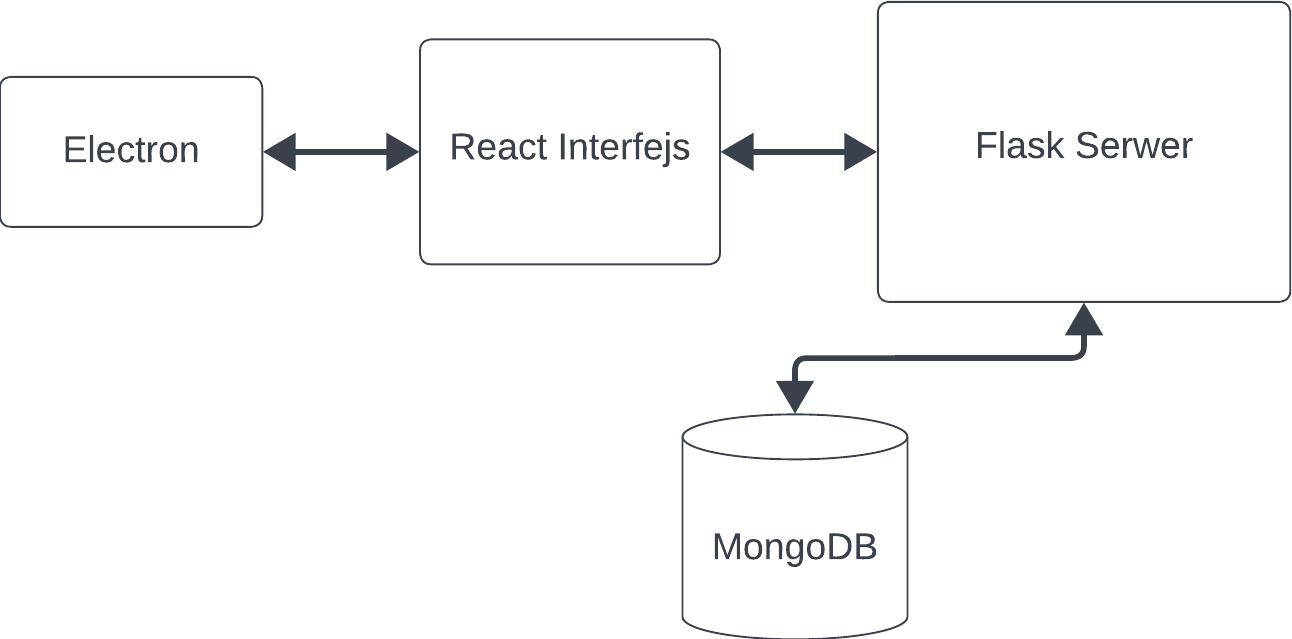
\includegraphics[width=\textwidth]{img/archi.png}
  \caption{Diagram łączenia komponentów}
\end{figure}
%% ########################################################
System składa się z 4 głównych komponentów:
\begin{enumerate}
	\item serwer HTTP - zbudowany z pomocą języka Python oraz biblioteki Flask,
	\item baza danych NoSQL
	\item interfejs użytkownika - generowany z użyciem frameworku Javascript React,
	\item konwerter na aplikację natywną Electron.
\end{enumerate}
Poniższe sekcje przedstawiają opis poszczególnych elementów służących do implementacji systemu. 
\subsubsection{Javascript React}
Jest to biblioteka pozwalająca na budowanie interaktywnych interfejsów użytkownika. Główną koncepcją React są komponenty, czyli samodzielne, hermetyczne jednostku interfejsu. Pozwala to na reakcje na zmiany wywołane przez użytkownika lub sam system i przy tym automatyczne aktualizowanie tych stron. React używa składni JSX (\textit{Javascript XML}), który jest rozszerzeniem składni Javascript. Integruje ona kod Javascript z deklaratywnym opisem struktury interfejsu.\par
React posiada specyficzne dla siebie struktury jakimi są ``\textit{hooks}''. Są to funkcje pozwalające na korzystanie z React, bez potrzeby tworzenia klas. Posiada on kilka wbudowanych funkcji tego rodzaju. Jedną z nich jest funkcja ``\textit{useState()}, która deklaruje zmienną stanu z wnętrza komponentu funkcyjnego. Jest to sposób na przechowanie wartości między wywołaniami funkcji. \par
Komunikacja z serwerem aplikacji odbywa się odbywa się z użyciem klienta HTTP \textit{Axios}, który jest mechanizmem opartym o obietnice (\textit{ang. promise}), co pozwala na asynchroniczną relację z punktem końcowym (\textit{ang. endpoint}). W systemie, po otrzymaniu odpowiedzi od serwera, ustawiany jest stan, czego przykład wykorzystania jest przedstawiony poniżej.
\begin{figure}[h!]
\centering
  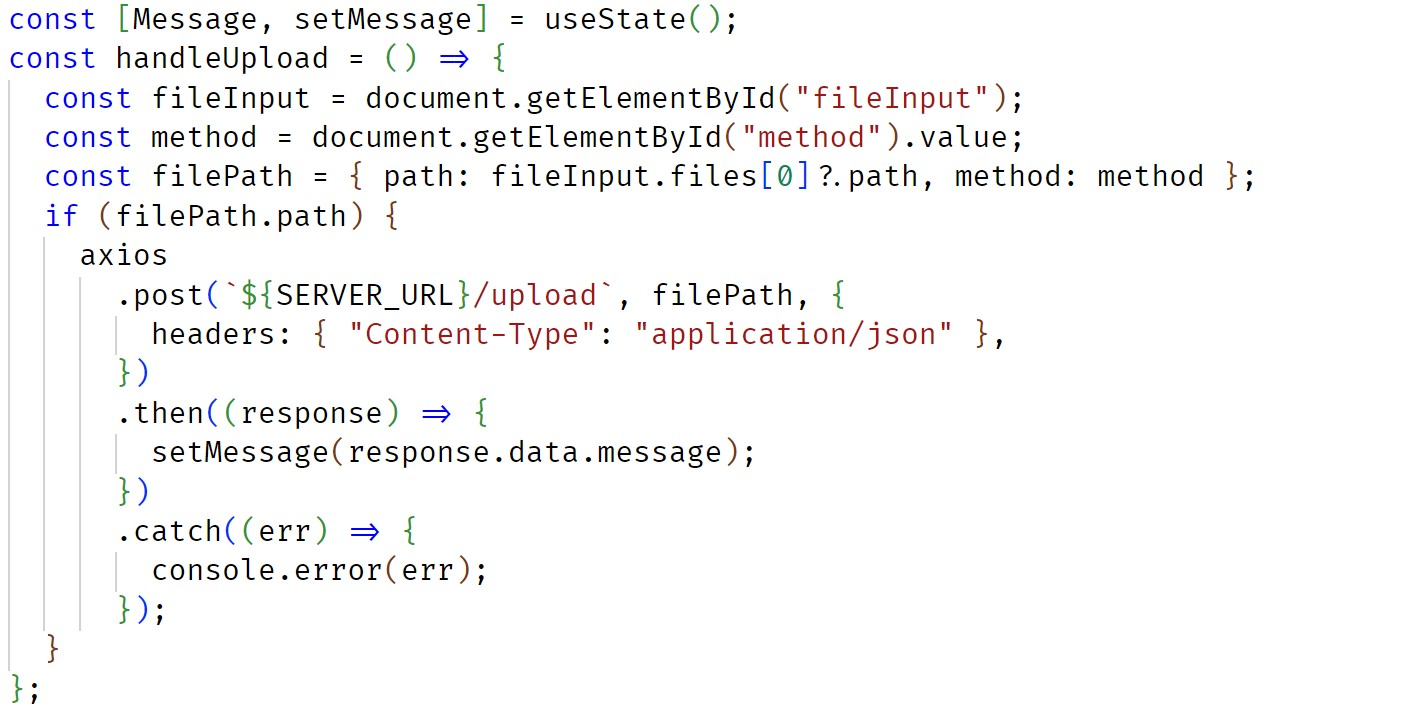
\includegraphics[width=\textwidth]{img/axios.jpg}
  \caption{Przykład wykorzystania \textit{Axios}; Implementacja dodania pliku}
\end{figure}
\subsubsection{Python Flask}
Flask jest to elastyczny framework, pozwalający na tworzenie aplikacji internetowych przy minimalnej ilości kodu. Dostarcza on jedynie niezbędne narzędzia, stawiając tym na dużą swobodę implementacji innych funkcji. 
Funkcja serwera jest uruchamiana w sytuacji gdy na podany adres URL zostanie wysłany komunikat. Informacja o aktywującym adresie jest przekazywana z użyciem dekoratora \textit{.route()}. Rysunek X przedstawia przykład takiego wywołania.\par
Jedną z możliwość tej biblioteki jest generowanie plików strony jako wynik końcowy działania funkcji. Kożystamy w takiej sytuacji z metody \textit{render\_template()}, która otrzymuje na wejściu uprzednio utworzony szablon HTML.\par 
Implementacja serwera z pomocą pakietu Flask umożliwia dostęp do szerokiego spektrum bibliotek języka Python, dotyczących sztucznej inteligencji i przetwarzania danych. 
\begin{figure}[h!]
\centering
  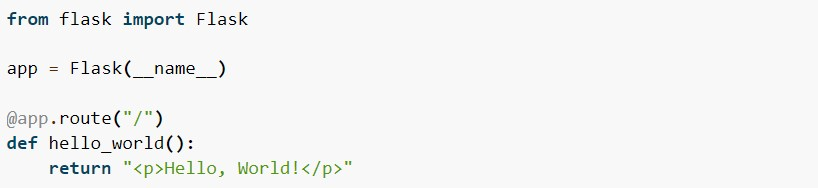
\includegraphics[width=\textwidth]{img/flask.jpg}
  \caption{Przykładowa implementacja funkcji serwera}
\end{figure}
%\begin{figure}[h!]
%\centering
%  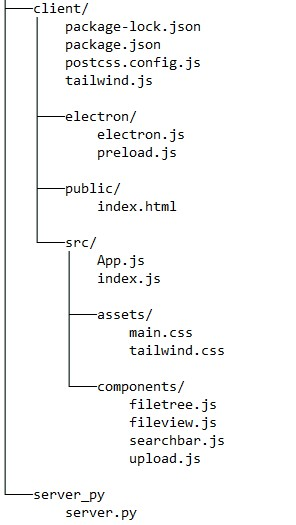
\includegraphics{img/file_structure.jpg}
%  \caption{Uogólniona struktura projektu}
%\end{figure}
%\newpage
%% ########################################################
\subsection{Obsługiwane rodzaje plików}
%% ########################################################
System jest przystosowany do obsługi plików o rozszerzeniach takich jak \textit{PDF}, \textit{CSV} i \textit{TXT}. Każdy rodzaj pliku ma osobne funkcjonalności opisane poniżej. Do plików przypisujemy tag opisujący rodzaj pliku, lecz jest on odrębną jednostką od słów kluczowych generowanych na podstawie zawartości pliku.
\subsubsection*{Pliki PDF}
Proces obsługi plików PDF jest zależny od wielu czynników. Najprostrzymi plikami do analizy są artykuły posiadające zakładki (\textit{ang. outlines}) o ujednoliconej strukturze, zawierające jedynie tekst. Słowo \textit{outlines} jest zwrotem specyficznym dla plików PDF i są potrzebne do ustalenia tytułu danego pliku. Wynika to z faktu, że nie zawsze nazwa pliku koresponduje tytułowi zawartości.\par
System wykorzystuje potokowanie zawartości w celu ekstrakcji tekstu, obrazów oraz tabel. Oznacza to, że aplikacja nie ``widzi'' dokumentu, lecz pobiera informacje z kodu źródłowego pliku. Działanie aplikacji jest oparte o sam tekst. Na potrzeby aplikacji, takie fragmenty jak tabele czy grafiki są jedynie przeszkodą, ponieważ nie powinne one wpływać na wynik algorytmu streszczania. Część elementów tabelarycznych jest niepoprawnie podpisywana jako tekst, co może przyczynić się do generacji niezrozumiałych streszczeń. 
\subsubsection*{Pliki tabelaryczne}
Podstawowym zachowaniem aplikacji w obliczu plików zawierających dane tabelaryczne jest generacja opisu zgodnie z następującymi krokami. Dla każdej kolumny pobierana jest jej nazwa oraz rodzaj danych zawartych w niej. Ze względu na specyfikę pliku, generacja słów kluczy może przebiec na dwa sposoby: tagami zostają nazwy kolumn lub użytkownik samodzielnie je dodaje.\par
Oba podejścia mają swoje wady. Nazwy kolumn nie są wymagane podczas kreacji tabel, więc tworzenie tagów w takiej sytuacji nie jest optymalne. Drugie podejście wymaga od użytkownika większego wkładu w ten proces. Potrzebna do tego jest pewna znajomość zestawu danych, który chcemy wprowadzić do systemu aby odpowiednio przypisać słowa klucze do plików.
\subsubsection*{Pliki tekstowe TXT}
Zawartość plików tekstowych nie jest uwarunkowana żadnymi normami, co czyni obsługę tych plików niemożliwą do standaryzacji. Podczas dodawania do aplikacji, wymagają one od użytkownika określenia rodzaju zawartości. Opcjami, które użytkownik ma do wyboru są: tekst lub dane tabelaryczne.\par
W pierwszym przypadku program sprawdza długość tekstu i na tej podstawie decyduje o następnych krokach. Domyślną długością graniczną jest 200 słów, lecz może ona być ustawiona manualnie przez klienta. Po przekroczeniu tego progu, system procesuje plik w sposób podobny do obsługi plików \textit{PDF}.\par
\subsection{Schematy poszczególnych funkcjonalności}
\subsubsection{Dodawanie plików PDF}
Zachowanie systemu przy dodaniu plików tekstowych.
\begin{enumerate}
	\item Gdy użytkownik wybierze plik, aplikacja przesyła ścieżkę pliku do serwera,
	\item System ekstraktuje z pliku całą zawartość z pomocą biblioteki języka Python \textit{PdfMiner},
	\item Z zawartości zostają wyciągnięte słowa klucze. Tworzenie tzw. tagów odbywa się z pomocą biblioteki \textit{yake} oraz metody \textit{KeywordExtractor()}. Przyjmuje ona następujące parametry:
	\begin{itemize}
		\item \textit{lan} - język danego tekstu,
		\item \textit{n} - maksymalna ilość słów w jednym tagu,
		\item \textit{deduplim} - szansa na powtóżenie się słów w różnych słowach kluczach,
		\item \textit{top} - ilość elementów wyjściowych
	\end{itemize}
	\begin{figure}[h]
		\centering
  		\includegraphics[width=\textwidth]{img/yake\_keyword.jpg}
  		\caption{Przykład użycia \textit{KeywordExtractor()}}
	\end{figure}
	\item w tym samym czasie z pomocą biblioteki \textit{sumy} oraz funkcji \textit{TextRankSummarizer}, jest tworzone streszczenie z użyciem algorytmu \textit{TextRank},
	\item jeżeli plik pdf posiada zakładki (ang. \textit{outlines}) to metoda \textit{.get\_outlines()} ekstraktuje je i z wyniku możemy otrzymać tytuł dokumentu i nadać plikowi taką nazwę. a jeżeli ich nie ma to tytułem pliku zostaje bazowa nazwa pliku,
	\item ostatecznie wszystkie informacje są zbierane i przesyłane do bazy danych.
\end{enumerate}
%\begin{figure}[h]
%\centering
%  \includegraphics[width=\textwidth]{img/file\_add\_pl.png}
%  \caption{Schemat sekwencyjny dodawania pliku}
%\end{figure}\par
Model TextRank zastosowany w projekcie, jest algorytmem rankingowym opartym na grafach \cite{textrank}. Operuje on na zasadach ``głosowania'' i ``rekomendacji''. Jest on używany do tworzenia streszczeń metodą ekstraktywną i nienadzorowaną. Dla przedstawionego systemu, nie jest możliwe wytworzenie odpowiedniego zbioru treningowego, aby móc zastosować metody nadzorowane. \par
Poniższy diagram przedstawia proces dodawania pliku PDF wraz z uwzględnieniem implementacji asocjacji plików o podobnej tematyce, opisanej w punkcie 2.4.3.
\begin{figure}[h!]
\centering
%  \includegraphics{img/activity\_diagram.png}
  \includegraphics{img/activity\_file\_add.png}
  \caption{Diagram aktywności przesyłania pliku PDF}
\end{figure}
\subsubsection{Wyszukiwanie i wyświetlanie plików}
Użytkownik ma możliwość wysukiwania plików po słowach kluczach lub tytule pliku. Tutaj przydatne jest użycie API generującego synonimy dla wyszukiwanego słowa. System zachowuje się w poniżej opisany sposób.
\begin{enumerate}
	\item aplikacja przesyła komunikat z wyszukiwanym słowem,
	\item serwer używając API synonimów pobiera 5 najbliższych słów do słowa szukanego,
	\item serwer przesyła osobne komunikaty do tabeli \textit{file\_properties} w bazie danych, zawierające osobno słowo klucz oraz synonimy
	\item baza zwraca informacje dotyczące znalezionych dokumentów oraz słowo klucz,
	\item serwer wysyła użytkownikowi posortowaną listę plików.
\end{enumerate}
\begin{figure}[h!]
\centering
  \includegraphics[width=\textwidth]{img/file\_search.png}
  \caption{Schemat sekwencyjny wyszukiwania pliku}
\end{figure}
\begin{figure}[h!]
\centering
  \includegraphics[width=\textwidth]{img/file\_search\_code.jpg}
  \caption{Implementacja wyszukiwania pliku}
\end{figure}
\newpage
\subsubsection{Obsługa plików zawierających dane tabelaryczne}
\begin{enumerate}
	\item użytkownik przy dodaniu pliku podaje następujące informacje:
	\begin{itemize}
		\item czy plik zawiera informacje o nazwach kolumn, jeżeli nie to czy chce on nadać te nazwy,
		\item czy słowa kluczowe będą nadane manualnie lub czy powinny być pobrane z nazw kolumn,
	\end{itemize}
	\item odpowiednio wczytywana na server do postaci ramki danych (\textit{ang. dataframe}) modułu \textit{pandas},
	\item sprawdzany i zapisywany jest typ wartości w każdej kolumnie oraz obliczony procent ilości wartości brakujących,
	\item dodanie rekordu do bazy danych.
\end{enumerate}
\begin{figure}[h!]
\centering
  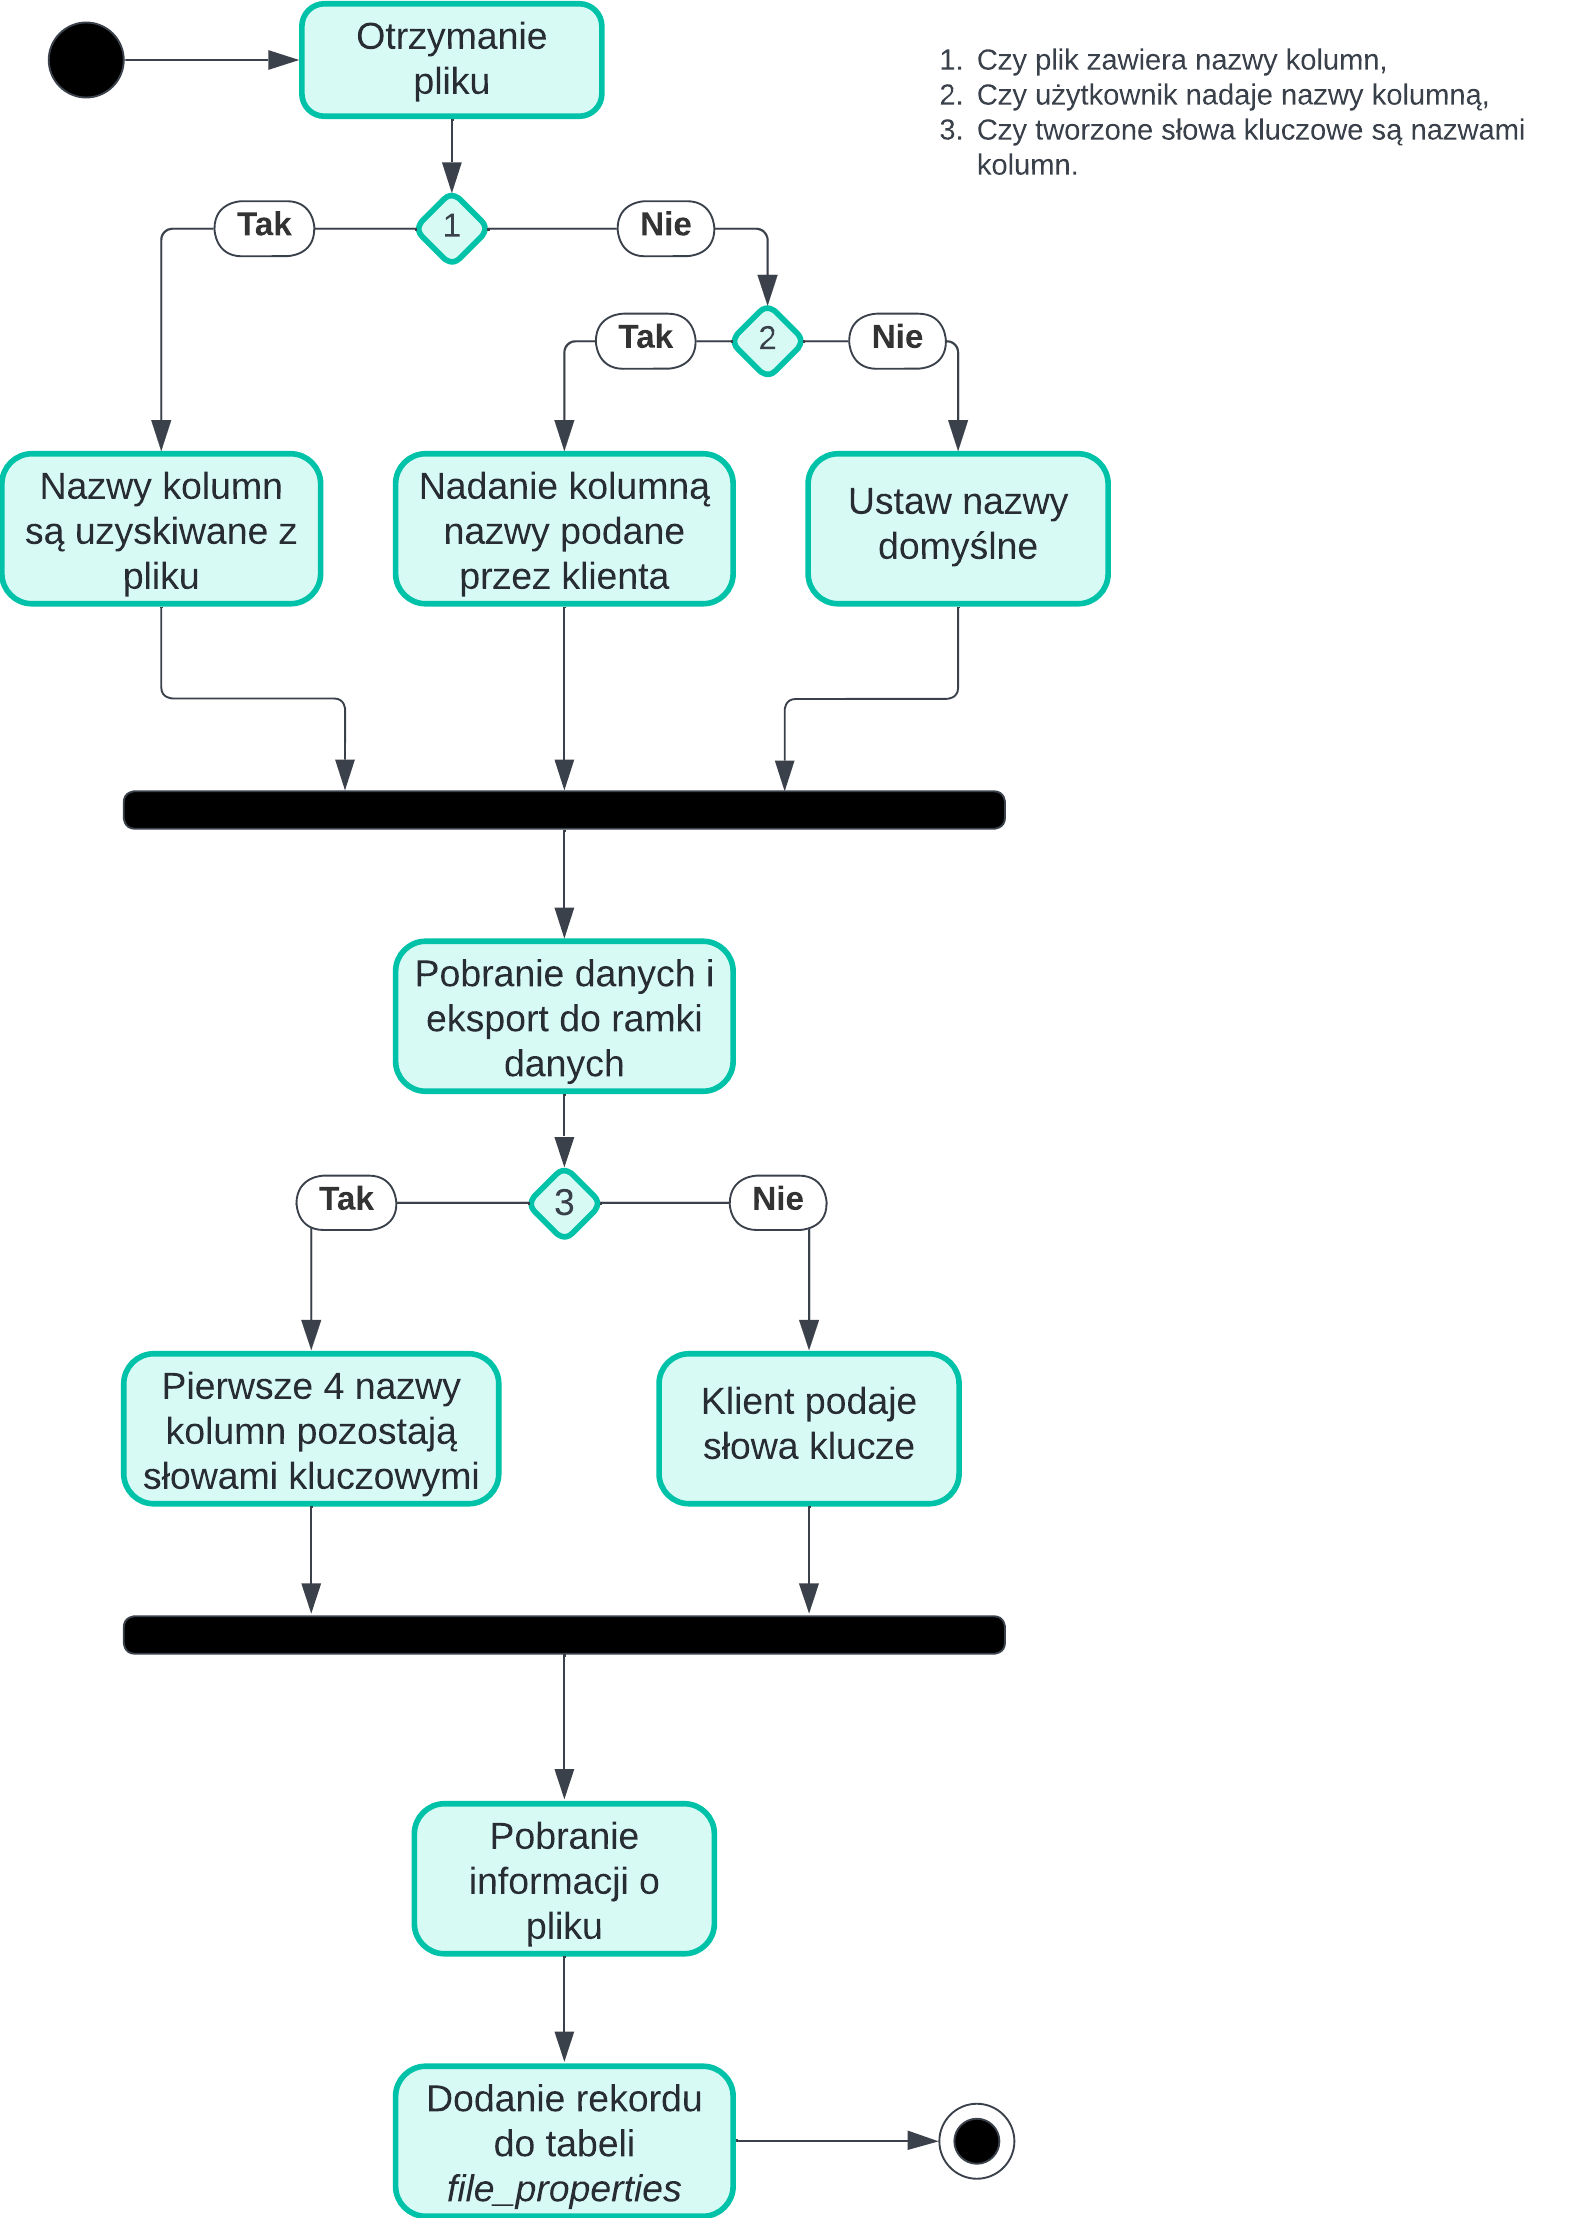
\includegraphics[width=\textwidth]{img/csvac.png}
  \caption{Diagram aktywności przetwarzania plików tabelarycznych}
\end{figure}
%% ########################################################
\clearpage
\newpage
\subsubsection{Asocjacja plików o podobnej tematyce}
Poniższa sekcja przedstawia proces łączenia dokumentów na podstawie wygenerowanych słów kluczowych. System z każdym dodanym plikiem przeszukuje przestrzeń dokumentów i aktualizuje już utworzone rekordy, w sytuacji dopasowania. Schemat przedstawia tworzenie połączeń dla nowo dodanego pliku.
\begin{enumerate}
\item dla każdego słowa kluczowego, jest pobrana lista ID plików z tabeli \textit{file\_properties}, pod warunkiem dopasowania przynajmniej jednego tagu,
\item następnie obliczany jest współczynnik podobieństwa, którego schemat postępowania jest przedstawiony poniżej:
	\begin{enumerate}
		\item wyznaczana jest wartość dla poszczególnych słów kluczy
		\begin{itemize}
			\item jeżeli wysłane słowo kluczowe zgadza się fragmentarycznie z otrzymanym tagiem (np. ``zaburzenia'' a ``zaburzenia odżywiania''), to zapisywana jest wartość $\frac{ilosc(dopasowan)}{ilosc\_slow(wejscie)+ilosc\_slow(pobrane)}$,
			\item jeżeli słowa są identyczne, zapisywana jest wartość 1,
		\end{itemize}
		\item wartości dla wszystkich słów kluczy są sumowane i dzielone przez liczbę tagów.
	\end{enumerate}
\item do ID pliku przypisana jest wartość podobieństwa, i po posortowaniu od największej wartości, ID są dodawane do jednego rekordu w tabeli \textit{file\_connections}
	\begin{itemize}
		\item jeżeli wartość podobieństwa nie przekracza 0.5, to plik nie jest brany pod uwagę
	\end{itemize}
\end{enumerate}
\newpage
\section{Możliwości rozwoju i wykorzystania aplikacji}
Wspomniane funkcjonalności to jedynie początek istnienia tego systemu. Stworzenie dodatkowych zdolności programu jest uproszczone, poprzez oparcie systemu o odpowiedzi w postaci komunikatu http zamiast stosowania szablonów, jak to jest zwykle przy standardowym projektowaniu z użyciem Python Flask. Baza danych wykorzystana w projekcie, MongoDB, jest bazą typu NoSQL, która umożliwia przechowywanie informacji w nie ustrukturyzowany sposób. Dzięki czemu tabele można wypełnić dowolnymi wartościami a sama aplikacja wyświetla wyszystkie elementy tabeli dla wyszukiwanego obiektu.\par
\subsection{Ekspansja działań dotyczących danych tabelarycznych}
Aktualny system pozwala na implementacje metod wstępnego przetwarzania danych (\textit{ang. preprocessing}) z wnętrza aplikacji. Preprocessing oznacza zbiór działań miejących na celu obróbkę i przygotowanie danych do dalszej manipulacji. Do takich działań należą usunięcie wartości brakujących, filtracja czy usuniecie wartości odstajacych. \par
Celem stworzenia systemu jest automatyzacja procesów związanych z przechowywaniem informacji. Dodanie takich możliwości jak łączenie tabel w pojedyńcze pliki czy w przypadku posiadania przez plik osobnych arkuszy danych pozwolenie na rozdzielenie ich na osobne pliki, powinno być celem kolejnych implementacji.
\subsection{Implementacja abstrakcyjnego tworzenia streszczeń}
Abstrakcyjna generacja streszczeń jest procesem wymagającym posiadania zestawu treningowego złożonych z streszczeń i przypisanym im tekstów początkowych. Jest to proces czasochłonny, lecz jakościowo przewyższa streszczenia metodami ekstraktywnymi. \par
Samodzielna kreacja takiego modelu nie jest optymalna pod względem ilości zasobów potrzebnych do modelowania a zasobów pamięciowych przeznaczonych na działanie całej aplikacji. Istnieje jednak rozwiązanie tego problemu za pomocą wykożystania \textit{API}. 
\subsection{Identyfikacja obrazów}
Identyfikacja obrazów mogą przysłużyć się sukcesowi systemu. Dla człowieka proces identyfikacji elementów obrazu dzieje się podświadomie, a w przypadku programu, jest on w stanie rozpoznać i przypisać grafikę do odpowiedniej kategorii, jedynie w sytuacji gdy jest on zaprogramowany do wykrywania ich. Komputery kategoryzują obrazy, porównując układ pikseli wejściowego obrazu ze schematami zapisanymi w systemie. Z punktu widzenia maszyny, obraz jest ustrukturyzowaną macierzą liczb, której każdy element zawiera informacje o nasyceniu i kolorze piksela. Aby stworzyć system odpowiedzialny za kategoryzację obrazów, należy przejść przez następujące kroki.
\begin{enumerate}
	\item Gromadzenie danych,
	\item Przygotowanie danych,
	\item Wybór, trenowanie i testowanie modelu,
	\item Wprowadzenie modelu do systemu.
\end{enumerate}
Najważniejszym elementem skutecznego systemu rozpoznawania obrazów jest dobrze skonstruowany zbiór danych. Etap gromadzenia danych obejmuje pozyskiwanie różnorodnych obrazów reprezentujących obiekty, sceny lub wzorce, które system nauczy się rozpoznawać. Kompleksowy zbiór danych przyczynia się do zdolności systemu do uogólniania swojego zrozumienia w różnych scenariuszach.\par
Przygotowanie danych (\textit{ang. Preprocessing}) to proces przekształcania i udoskonalania zebranych danych, aby były odpowiednie do przeprowadzenia treningu systemu. Może to obejmować takie zadania, jak usuwanie niespójności, zmiana rozmiaru obrazów do spójnego formatu i normalizacja wartości pikseli. Skuteczny preprocessing danych wspomaga zdolność modelu do nauki istotnych wzorców z danych.\par
Kluczową decyzją jest wybór architektury modelu. Wybór architektury powinien być dostosowany do wymagań zadania i zasobów obliczeniowych. Określa ona sposób, w jaki system będzie przetwarzał i interpretował dane wejściowe. Trening modelu to proces uczenia wybranej architektury rozpoznawania wzorców i cech w danych treningowych. Osiąga się to poprzez iteracyjną optymalizację, w której parametry modelu są dostosowywane w celu zminimalizowania różnicy między przewidywanymi a rzeczywistymi wynikami. Trening trwa do momentu, aż model osiągnie optymalny poziom dokładności i uogólnienia, który sprawi, że będzie on biegły w rozpoznawaniu obiektów na obrazach. \par
Ostatnim etapem, poprzedzającym implementacje modelu, jest testowanie wytrenowanego modelu. Jest ono niezbędne do oceny jego wydajności dla nowych danych. System jest zasilany obrazami, których nie napotkał podczas szkolenia, umożliwiając ocenę jego zdolności do generalizacji. Metryki takie jak dokładność, precyzja i czułość zapewniają wgląd w mocne i słabe strony modelu. Rygorystyczne testowanie pomaga w dostrojeniu modelu w celu uzyskania lepszej wydajności.\par
Powszechnie dostępne, ogromne bazy danych, takie jak \textit{Pascal VOC} czy \textit{ImageNet}, pozwalają na stworzenie i wdrożenie takiego modelu. Zawierają one mnóstwo oznaczonych wzorców opisujących obiekty znajdujące sie na obrazach. 
%% ########################################################
%\subsection{Kategoryzowanie plików względem zawartości}
%Na obecnym etapie implementacji systemu, wszystkie pliki znajdują się w jednym miejscu oraz jedynym sposobem na odnalezienie plików jest skorzystanie z zaprogramowanej wyszukiwarki plików. System łączy pliki ze względu na wspólne słowa klucze, lecz nie ingeruje w proces sytuowania obiektów w katalogu aplikacji. Pliki o różnorodnej tematyce mieszają się ze sobą do tego stopnia, że nie jest możliwe, aby przy niepoprawnie nazwanych plikach, znaleźć te potrzebne. \par
%Odpowiedzią na ten problem jest system kategoryzacji i podziału plików. Segregacja powinna odbywać się na podstawie słów kluczy, jednakże dalsze badania są wymagane do określenia wymagań warunku podziału. Niepoprawny warunek może spowodować duplikację plików na szeroką skalę, co negowałoby cel tej implementacji.
%% ########################################################
\section*{Podsumowanie}
\addcontentsline{toc}{section}{Podsumowanie}
W ramach projektu zaimplementowano aplikację umożliwiającą komfortowe przechowywanie oraz zmniejszenie ingerencji użytkownika w proces interpretacji plików. Opisano funkcjonalności aplikacji oraz możliwe rozszerzenia  aplikacji w dalszym ciągu rozwoju. \par
Badania nad aplikacją wyeksponowały ciekawy koncept jakim jest praca z pilkami o rozszerzeniu PDF, jakoże proces automatycznego pobierania tekstu jest zależny od wielu czynników. Okazało się, że rozkład tekstu na stronie jak i program, którego użyto do stworzenia pliku może przyczynić się do błędnego eksportu tekstu. Nie jest możliwe uwzględnienie każdego przypadku stuktury pliku aby zapewnić prawidłowy proces ekstrakcji. Należałoby zastanowić się nad poprawą implementacji tego algorytmu lub zastosowanie innych sposobów, takich jak \textit{Optical Character Recognition}. System powinien być usprawniony o implementacje serwera HTTP oraz logowanie, aby zezwolić na przenoszenie danych użytkownika.
%% ########################################################
\newpage
\listoffigures
\addcontentsline{toc}{section}{Spis Rysunków}
\addcontentsline{toc}{section}{Bibliografia}
\bibliographystyle{IEEEtran}
\bibliography{biblioteka}
\end{document}